

\chapter{Basics of model rocket flight}
\label{chap-basics}


As rockets and rocket motors come in a huge variety of shapes and
sizes, different categories are defined for different levels of
rocketry.  {\it Model rocketry} itself is governed by the NAR Model
Rocket Safety Code~\cite{nar-safety-code} in the U.S. and other
similar regulations in other countries.  The safety code requires that
the model rockets be constructed only of light-weight materials
without any metal structural parts, and have a maximum lift-off weight
of 1.5~kg.  They may only used pre-manufactured motors of classes A--G
(see Section~\ref{sec-motor-classes} for the classification).

{\it High power rocketry} (HPR) is basically scaled up model
rocketry.  There are no weight restrictions, and they can use
pre-manufactured solid or hybrid rocket motors in the range of H--O.
The combined total impulse of all motors may not exceed 81\s920~Ns.

{\it Experimental} or {\it amateur rocketry} includes any rocketry
activities beyond model and high power rocketry.  This may include
for example using motor combinations that exceed the limits placed by
high power rocketry, building self-made motors or utilizing liquid
fueled motors. Finally there is {\it professional rocketry} which is
conducted for profit, usually by governments or large corporations.

Even though rockets come in many different sizes, the same principles
apply to all of them.  In this thesis the emphasis will be on model
rocketry, but the results are just as valid for larger rockets as long
as the assumptions of for example the speed range remain valid.  In
this chapter the basics of model rocketry and differences to high
power rocketry are explained.


\section{Model rocket flight}

A typical flight of a model rocket can be characterized by the four
phases depicted in Figure~\ref{fig-model-flight}:
%
\begin{enumerate}
\item Launch:  The model rocket is launched from a vertical launch
  guide.
\item Powered flight:  The motor accelerates the rocket during the
  powered flight period.
\item Coasting flight:  The rocket coasts freely until approximately
  at its apogee.
\item Recovery:  The recovery device opens and the rocket descends
  slowly to the ground.
\end{enumerate}

\begin{figure}
\centering
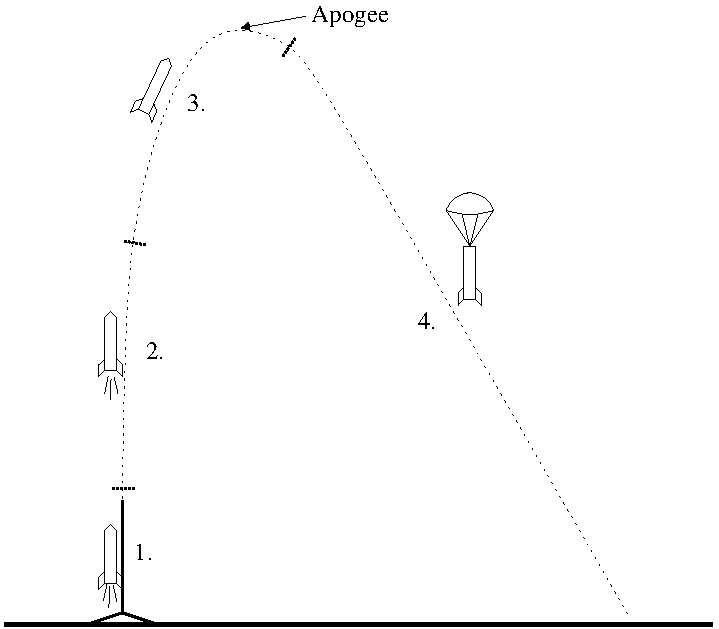
\epsfig{file=figures/model-flight,scale=0.8}
\caption{The basic phases of a typical model rocket flight:
  1.~Launch, 2.~Powered flight, 3.~Coasting and 4.~Recovery.}
\label{fig-model-flight}
\end{figure}

Model rockets are launched from a vertical launch guide that keeps the
rocket in an upright position until it has sufficient velocity for the
fins to aerodynamically stabilize the flight.  The NAR safety code
forbids launching a model rocket at an angle greater than 
$30^\circ$ from vertical.  A typical launch guide for small rockets is
a metal rod about 3-5~mm in diameter, and the launch lug is a short
piece of plastic tube glued to the body tube.  Especially in 
larger rockets this may be replaced by two extruding bolts, the ends
of which slide along a metal rail.  Use of a launch lug can be avoided
by a tower launcher, which has 3--4 metal bars around the rocket
that hold it in an upright position.

After clearing the launch guide, the rocket is in free, powered flight.
During this phase the motor accelerates the rocket while it is
aerodynamically stabilized to keep its vertical orientation.  When the
propellant has been used, the rocket is typically at its maximum
velocity.  It then coasts freely for a short period while the motor
produces smoke to help follow the rocket, but provides no
additional thrust.  Finally, at approximately the point of apogee, a
small pyrotechnical ejection charge is fired upwards from the motor
which pressurizes the model rocket and opens the recovery device.

High-power rocket motors usually have no ejection charges incorporated
in them.  Instead, the rocket carries a small flight computer that
measures the acceleration of the rocket or the outside pressure change
to detect the point of apogee and to open the recovery device.
Frequently only a small drogue parachute is opened at apogee, and the
main parachute is opened at some pre-defined lower altitude around
100--300 meters.

The typical recovery device of a model rocket is either a parachute or
a {\it streamer}.  The parachutes are usually a simple planar circle
of plastic or fabric with 4--10 shroud lines attached.  A streamer is
a strip of plastic or fabric connected to the rocket, intended to
flutter in the air and thus slow down the descent of the rocket.
Especially small rockets often use streamers as their recovery device,
since even light wind can cause a light-weight rocket with a
parachute to drift a significant distance.




\section{Rocket motor classification}
\label{sec-motors}
\label{sec-motor-classes}

The motors used in model and high power rocketry are categorized based
on their total impulse.  A class `A' motor may have a total impulse in
the range of 1.26--2.50~Ns.  Every consecutive class doubles the
allowed total impulse of the motor.  Thus, a B-motor can have an
impulse in the range 2.51--5.00~Ns and a C-motor in the range
5.01--10.0~Ns.  There are also classes \half A and \quarter A which
have impulse ranges half and one quarter of those of an A-motor,
respectively.  Commercial rocket motors are available up to
class~O with a total impulse of 30\s000~Ns~\cite{all-certified-motors}.
Table~\ref{tab-motor-classes} lists the impulse ranges for model
and high-power rocket motors. 

\begin{table}
\caption{Total impulse ranges for motor classes \quarter A--O.}
\label{tab-motor-classes}
\begin{center}
\begin{tabular}{cr@{--}l|cr@{--}l|cr@{--}l}
\hline
\quarter A & 0.0 & 0.625~Ns   & E & 20.01 & 40.0~Ns & K & 1280.01 & 2560~Ns \\
\half A & 0.626 & 1.25~Ns  & F & 40.01 & 80.0~Ns & L & 2560.01 & 5120~Ns \\
A    & 1.26 & 2.50~Ns   & G & 80.01 & 160~Ns  & M & 5120.01 & 10240~Ns \\
B    & 2.51 & 5.00~Ns   & H & 160.01 & 320~Ns   & N & 10240.01 & 20480~Ns \\
C    & 5.01 & 10.0~Ns   & I & 320.01 & 640~Ns   & O & 20480.01 & 40960~Ns \\
D    & 10.01 & 20.0~Ns  & J & 640.01 & 1280~Ns  &  \\
\hline
\end{tabular}
\end{center}
\end{table}

Another important parameter of a rocket motor is the thrust given by
the motor.  This defines the mass that may be lifted by the motor and
the acceleration achieved.  Small model rocket motors typically have
an average thrust of about 3--10~N, while high-power rocket motors can
have thrusts in excess of 5\s000~N.

The third parameter used to classify a model rocket motor is the
length of the delay between the motor burnout and the ignition of the
ejection charge.  Since the maximum velocity of different rockets
using the same type of motor can be vastly different, also the length
of the coasting phase varies.  Therefore motors with otherwise the
same specifications are often manufactured with several different
delay lengths.  These delay lengths do not apply to high-power rocket
motors, since they do not have ejections charges incorporated in them.

Model rocket motors are given a classification code based on these
three parameters, for example ``D7-3''.  The letter specifies the
total impulse range of the motor, while the first number specifies the
average thrust in Newtons and the second number the delay of the
ejection charge in seconds.  The delay number can also be replaced by
`P', which stands for {\it plugged}, \ie the motor does not have an
ejection charge.  Some manufacturers may also use an additional letter
at the end of the classification code specifying the
propellant type used in the motor.

Even motors with the same classification code may have slight
variations to them.  First, the classification only specifies the
impulse range of the motor, not the exact impulse.  In principle, a
D-motor in the lower end of the range might have a total impulse only
1~Ns larger than a C-motor in the upper end of its range.  Second,
the code only specifies the average thrust of the motor.  The thrust
rarely is constant, but varies with time.
Figure~\ref{fig-thrust-curve} shows the typical thrust curve of a
small black powder rocket motor.  The motors typically have a short
thrust peak at ignition that gives the rocket an initial acceleration
boost before stabilizing to a thrust level a little below the average
thrust.  Statically measured thrust curves of most commercial rocket
motors are readily available on the
Internet~\cite{thrust-curve-database}.

\begin{figure}
\centering
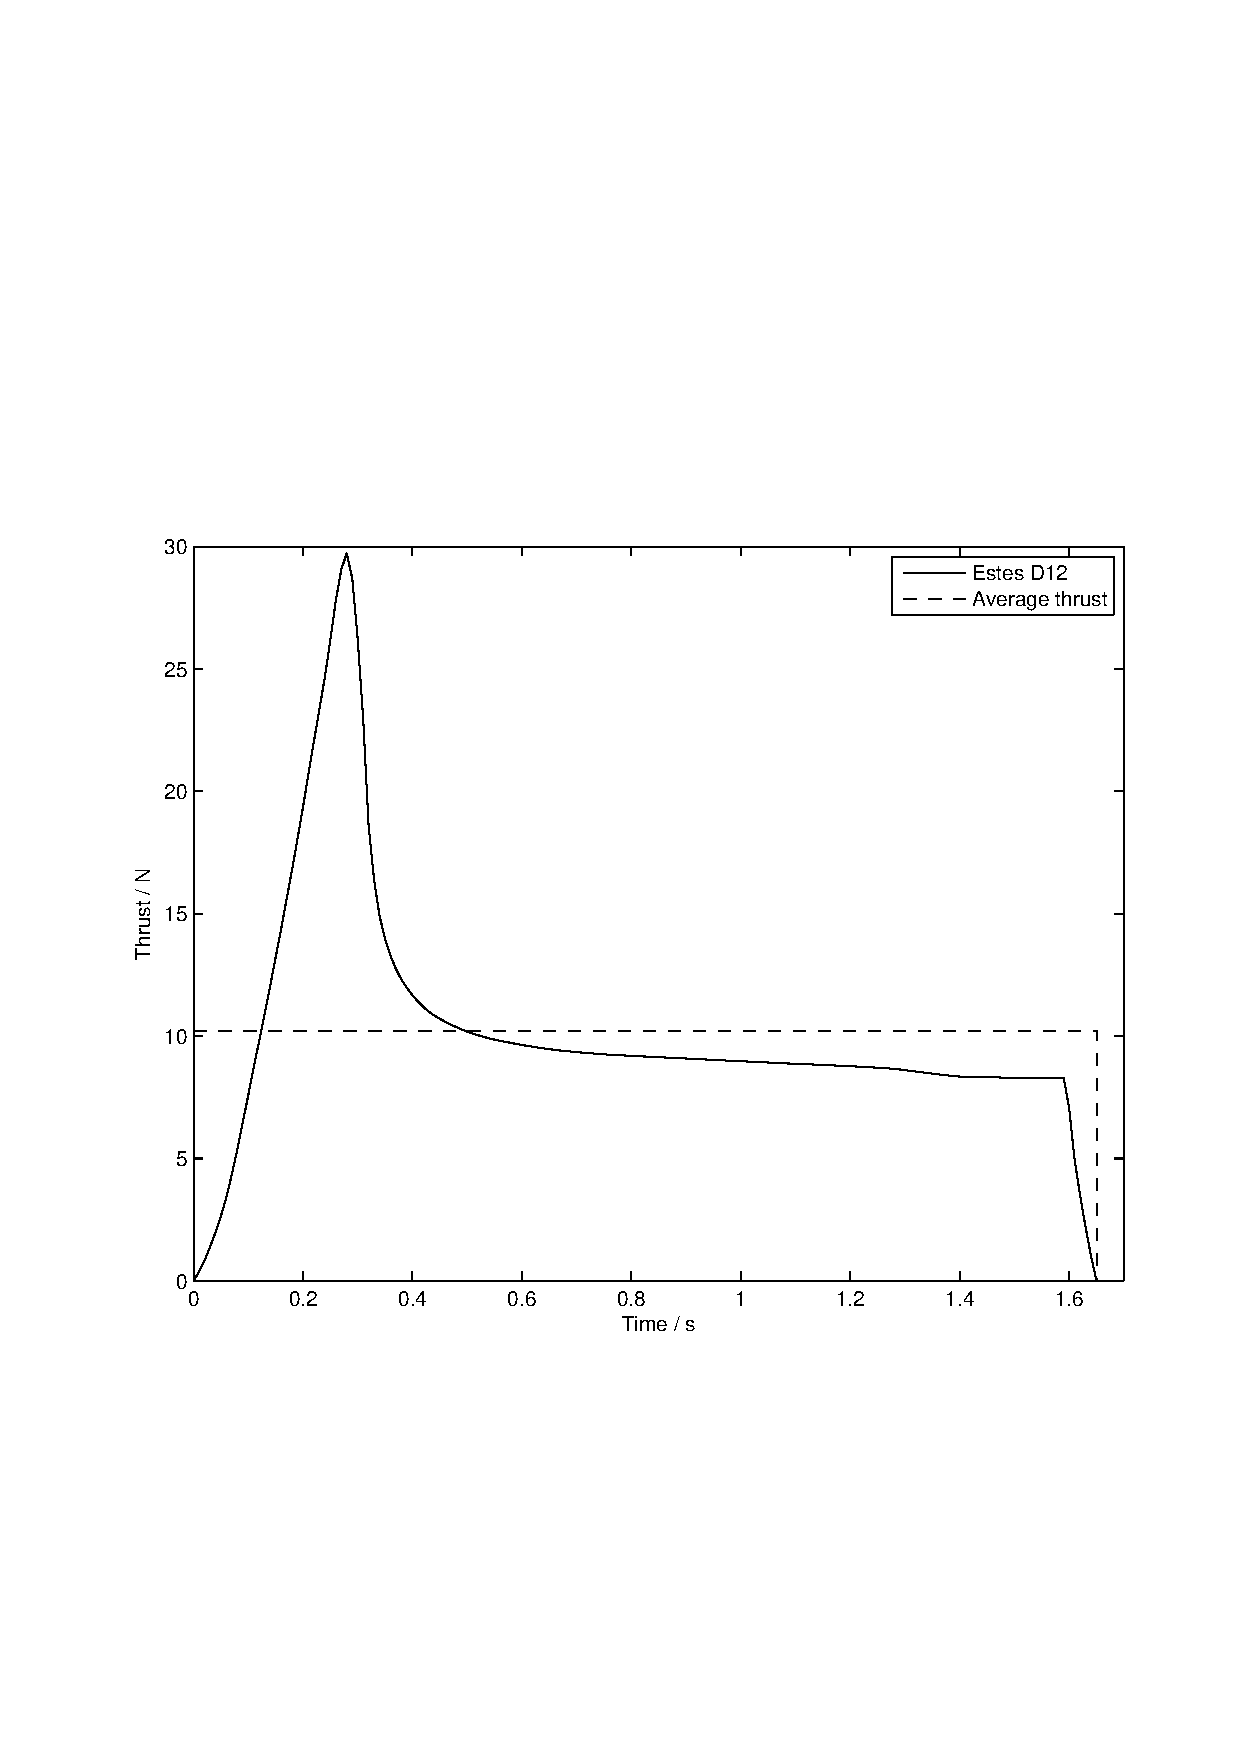
\epsfig{file=figures/motors/D12-thrustcurve,width=9cm}
\caption{A typical thrust curve of an Estes D12-3 rocket motor and
  its average thrust.~\cite{D12-curve}}
\label{fig-thrust-curve}
\end{figure}

Also the propellant type may affect the characteristics of the motor.
Most model rocket motors are made up of a solid, pyrotechnical
propellant---typically black powder---that is cast into a suitable
shape and ignited on launch.  Since the propellant burns on its
surface, different thrust curves can be achieved by different mold
shapes.

% vesiraketit!

A significantly different motor type, {\it hybrid motors}, were
commercially introduced in 1995.  These motors typically include the
propellant and oxidizer in different states, typically a composite
plastic as the fuel and a separate tank of liquid nitrous oxide 
($\rm N_2O$) as the oxidizer.  The plastic on its own does not 
burn very well, but provides ample thrust when the nitrous oxide is
fed through its core.  The nitrous oxide tank is
self-pressurized by its natural vapor pressure. However, since
temperature greatly affects the vapor pressure of nitrous oxide, the
thrust of a hybrid motor is also diminished if the oxidizer is cold.
On the other hand, the motor will burn longer in this case, and since
nitrous oxide is denser when cold, the motor may even yield a greater
total impulse.

The significance of this effect was observed when analyzing the video
footage of the launch of the first Finnish hybrid rocket,
``Haisun��t�''~\cite{haisunaata-launch}.  The average thrust during the
first 0.5~seconds was determined to be only about 70~N, whereas the
static tests suggest the thrust should have been over 200~N.
Instead, the motor burned for over 10~seconds, while the normal thrust
curves indicate a burning time of 5--6~seconds.  This shows that the
temperature of the hybrid motor oxidizer can have a dramatic effect on
the thrust given by the motor, and the static test curve should be
assumed to be valid only in similar operating conditions as during the
test.

One further non-pyrotechnical rocket type is {\it water rockets}.
These are especially popular first rockets, as they require no special
permits and are easy to construct.  The water rocket includes a bottle
or other chamber that has water and pressurized air inside it.  On
launch the pressure forces the water out of a nozzle, providing thrust
to the rocket.  While simulating water rockets is beyond the scope of
this thesis, it is the aim that methods for modeling water rockets can
be added to the produced software in the future.



\section{Clustering and staging}

Two common methods used to achieve greater altitudes with model
rockets are {\it clustering} and {\it staging}.  A cluster has two or
more rocket motors burning concurrently, while staging uses motors
that burn consecutively.  The motor configuration of a cluster and
staged rocket is depicted in Figure~\ref{fig-cluster-stages}.

When a cluster is launched, the total thrust is the sum of the thrust
curves of the separate motors.  This allows greater acceleration and
a greater liftoff weight.  Staging is usually performed by using
zero-delay motors, that ignite the ejection charge immediately at
burnout.  The ejection charge fires towards the upper stage motor and
ignites the next motor.  High power motors with no ejection charges
can be clustered by using an onboard accelerometer or timer that
ignites the subsequent stages.  Staging provides a longer duration of
powered flight, thus increasing the altitude.


\begin{figure}
\centering
\parbox{65mm}{\centering
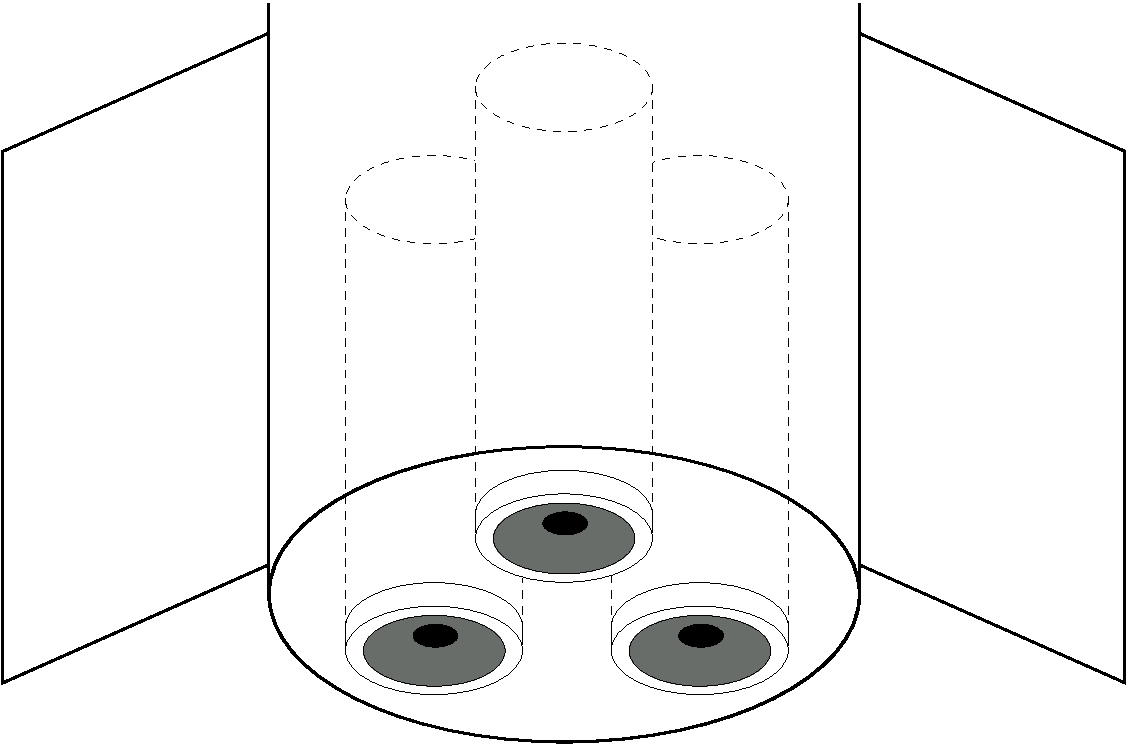
\epsfig{file=figures/motors/cluster,width=60mm} \\ (a)}
\hspace{10mm}
\parbox{40mm}{\centering
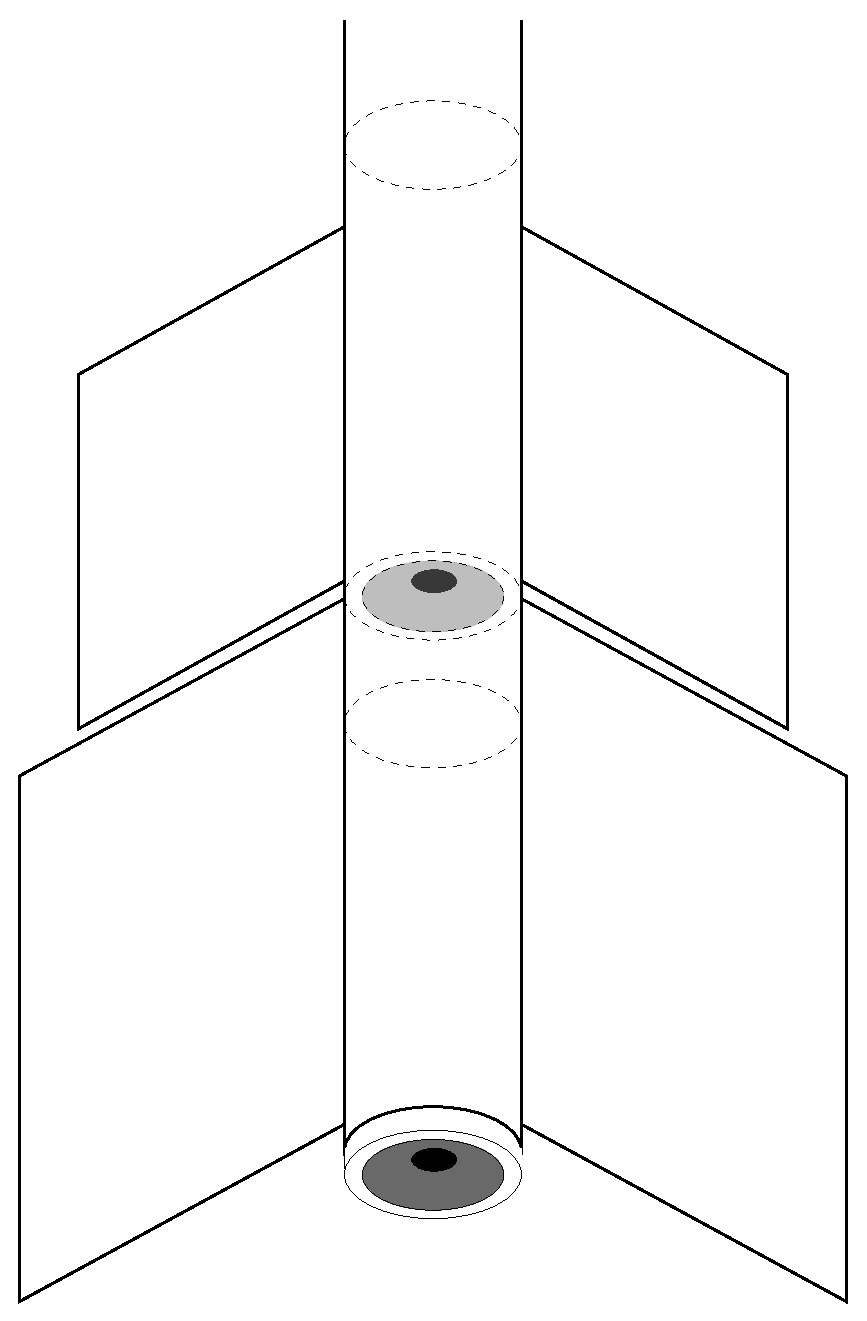
\epsfig{file=figures/motors/staged,width=30mm} \\ (b)}
\caption{The motor configuration for (a) a cluster rocket and (b) a
  two-staged rocket.}
\label{fig-cluster-stages}
\end{figure}

Clustering provides a greater acceleration at launch, but staging
typically provides greater altitude than a cluster with similar
motors.  This is because a clustered rocket accelerates quickly to a
greater speed thus also increasing the aerodynamic drag.  A staged
rocket has a smaller thrust for a longer period of time, which reduces
the overall effect of drag during the flight.


\section{Stability of a rocket}
\label{sec-stability}

When designing a new rocket, its stability is of paramount
importance.  A small gust of wind or some other disturbance may cause
the rocket to tilt slightly from its current orientation.  When this
occurs, the rocket centerline is no longer parallel to the
velocity of the rocket.  This condition is called flying at an 
{\it angle of attack $\alpha$}, where $\alpha$ is the angle between
the rocket centerline and the velocity vector.

When a stable rocket flies at an angle of attack, its fins produce a
moment to correct the rocket's flight.  The corrective moment is
produced by the aerodynamic forces perpendicular to the axis of the
rocket.  Each component of the rocket can be seen as producing a
separate normal force component originating from the component's CP,
as depicted in Figure~\ref{fig-normal-forces}.

\begin{figure}
\centering
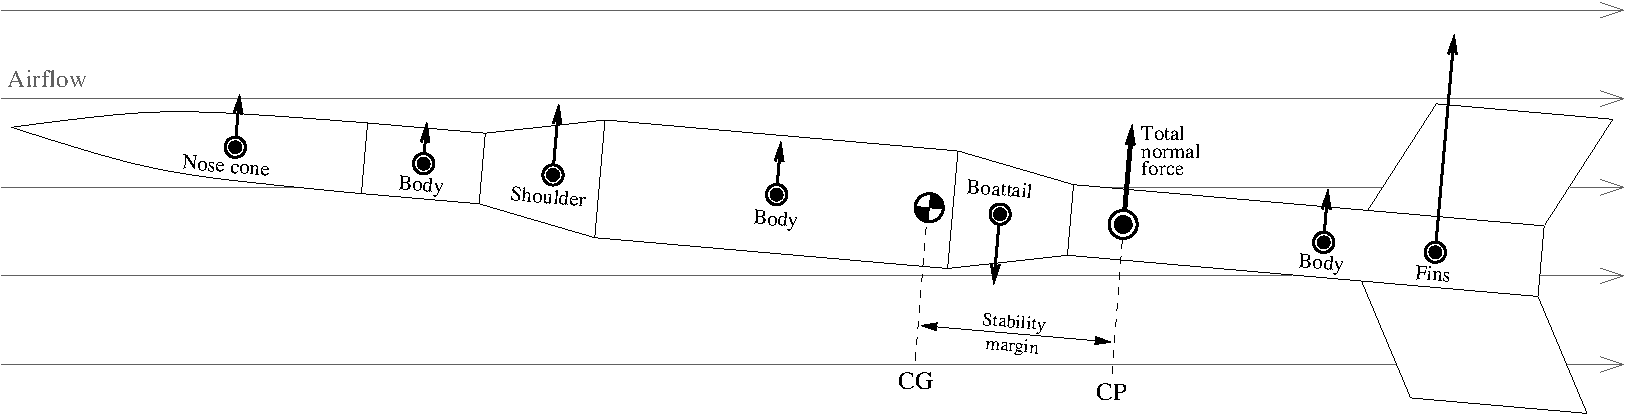
\epsfig{file=figures/aerodynamics/component-normal-forces,width=130mm}
\caption{Normal forces produced by the rocket components.}
\label{fig-normal-forces}
\end{figure}

The effect of the separate normal forces can be combined into a single
force, the magnitude of which is the sum of the separate forces and
which effects the same moment as the separate forces.  The point on
which the total force acts is defined as the center of pressure or the
rocket.  As
can be seen from Figure~\ref{fig-normal-forces}, the moment produced
attempts to correct the rocket's flight only if the CP is located aft
of the CG. If this condition holds, the rocket is said to be 
{\it statically stable}.  A statically stable rocket always produces a
corrective moment when flying at a small angle of attack.  

The argument for static stability above may fail in two conditions:
First, the normal forces might cancel each other out exactly, in which
case a moment would be produced but with zero total force.  Second,
the normal force at the CP might be in the wrong direction (downward
in the figure), yielding an uncorrective moment.  However, we shall
see that the only component to produce a downward force is a boattail,
and the force is equivalent to the corresponding broadening of the
body.  Therefore the total force acting on the rocket cannot be zero
nor in a direction to produce an uncorrective moment when aft of the
CG.

The {\it stability margin} of a rocket is defined as the distance between
the CP and CG, measured in {\it calibers}, where one caliber is the
maximum body diameter of the rocket.  A rule of thumb among model
rocketeers is that the CP should be approximately 1--2 calibers aft of
the CG.  However, the CP of a rocket typically moves upwards as the
angle of attack increases.  In some cases, a 1--2 caliber stability
margin may totally disappear at an angle of attack of only a few
degrees.  As side wind is the primary cause of angles of attack, this
effect is called 
{\it wind caused instability}~\cite{galejs}.

Another stability issue concerning rocketeers is the
{\it dynamic stability} of a rocket.  A rocket that is statically
stable may still be poor at returning the rocket to the original
orientation quickly enough.  Model rockets may encounter several types of
dynamic instability depending on their shape, size and
mass~\cite[pp.~140--141]{stine}:
%
\begin{enumerate}
\item {\it Too little oscillation damping.}  In short, light-weight
  rockets the corrective moment may significantly over-correct the
  perturbation, requiring a corrective moment in the opposite
  direction.  This may lead to continuous oscillation during the
  flight.
\item {\it Too small corrective moment.}  This is the case of over-damped
  oscillation, where the corrective moment is too small compared to
  the moment of inertia of the rocket.  Before the rocket has been
  able to correct its orientation, the thrust of the motors may have
  already significantly affected the direction of flight.
\item {\it Roll-pitch coupling.}  If the model has a natural roll
  frequency (caused \eg by canting the fins) close to the oscillation
  frequency of the rocket, roll-pitch resonance may occur and cause
  the model to go unstable.
\end{enumerate}

By definition, dynamic stability issues are such that they occur over
time during the flight of the rocket.  A full flight simulation that
takes into account all corrective moments automatically also simulates
the possible dynamic stability problems.  Therefore the dynamic
stability of rockets will not be further considered in this
thesis. For an analytical consideration of the problem, refer to
\cite{advanced-model-rocketry}.



